\chapter{Linked Lists} \label{chp:linkedlist}
\epigraph{Where did you come from, where did you go? // Where did you come from, Cotton-Eye Joe?}
{Rednex}

Unsere Arbeit mit Listen involvierte bislang immer Arrays. Dies ist günstig, solange wir die Liste nicht vergrößern oder verkleinern wollen. Soll aber ein Element an die Liste angehängt werden, kann dies ein sehr ungünstiges \emph{Laufzeitverhalten}\footnote{Das Laufzeitverhalten ist ein Maß für den Zeitbedarf eines Algorithmus, in Abhängigkeit von der zu verarbeitenden Datenmenge. Wenn eine Liste mit \texttt{n} Elementen mit dem Befehl \texttt{realloc} vergrößert werden soll, kann es sein, dass diese \texttt{n} Werte an eine andere Stelle im Speicher \enquote{umgezogen} werden müssen. Dieses Umziehen bedeutet Kopieren und kostet Zeit, und zwar für jedes Listenelement. Je länger die Liste ist, desto mehr Zeit kann das \texttt{realloc} also beanspruchen.} erzeugen. Noch schwieriger wird es, wenn ein neues Element \emph{in der Mitte der Liste} eingefügt werden soll.

In diesem Kapitel werden wir eine Datenstruktur kennenlernen, die bei Einfügungen und Löschung aus der Liste ein wesentlich besseres Laufzeitverhalten zeigt.

\section{Ausgangslage: Klassische Arrays}
\begin{codebox}[Beispiel: Einfügen in eine Liste: Lösung mit Arrays]
\begin{minted}[linenos]{c}
#include <stdio.h>
#include <stdlib.h>

int * insert_into_list(int * list, int N, int newVal, int pos) {
  if (pos<0) {printf("Fehler: Einfügung vor dem Listenanfang\n");  return NULL;}
  if (pos>N) {printf("Fehler: Einfügung hinter dem Listenende\n"); return NULL;}
  
  int * newlist = malloc((N + 1) * sizeof(*newlist));
  if (!newlist) {printf("Fehler: Allozierung fehlgeschlagen\n");   return NULL;}
  
  for (int i=0; i<pos; i++) {
    newlist[i] = list[i];
  }

  newlist[pos] = newVal;

  for (int i=pos+1; i<N+1; i++) {
    newlist[i] = list[i-1];
  }
  
  free(list);
  return newlist;
}
\end{minted}
\end{codebox}
%
\begin{codebox}[]
\begin{minted}[linenos, firstnumber=last]{c}
void print_list(int * list, int N) {
  for (int i=0; i<N; i++) {
    printf("Element #%d: %3d\n", i, list[i]);
  }
}

int main() {
  int N = 5;
  int * list = malloc(N * sizeof(*list));
  
  if (!list) {
    printf("Fehler: Allozierung fehlgeschlagen\n");
    return -1;
  }
  
  for (int i=0; i<N; i++) {
    list[i] = i;
  }
  
  printf("vorher:\n");
  print_list(list, N);
  
  
  int * dummy = insert_into_list(list, N, 666, 3);
  if (dummy) {list = dummy; N++;}
  else       {printf("Keine Einfügung hat stattgefunden.\n");}
  
  printf("nachher:\n");
  printlist(list, N);
  
  free(list);
  return 0;
}
\end{minted}
\end{codebox}

\begin{cmdbox}[Ausgabebeispiel: Einfügen in eine Liste: Lösung mit Arrays]
vorher:\\
Element \#0:   0\\
Element \#1:   1\\
Element \#2:   2\\
Element \#3:   3\\
Element \#4:   4\\
nachher:\\
Element \#0:   0\\
Element \#1:   1\\
Element \#2:   2\\
Element \#3: 666\\
Element \#4:   3\\
Element \#5:   4
\end{cmdbox}
Wir legen hier in der \texttt{main} ein dynamisches Array mit \texttt{N=5} Elementen an, und befüllen Sie mit Beispieldaten, hier aufsteigend die Werte \texttt{0\ldots N-1}. Die Funktion 
\texttt{insert\_into\_list} fügt dann an vierter Stelle (Arrayindex \texttt{3}) einen neuen Wert ein.

Dieses Einfügen geschieht, indem eine \emph{Kopie der Original-Liste} angelegt wird. Diese Kopie geht aber nur bis zum Listenelement \texttt{pos}, also bis zu der Stelle, an der ein neues Element in die Liste eingefügt werden soll. Ebenso werden die Listenelemente mit den Indizes \texttt{pos\ldots N-1} kopiert, jedoch mit einem \emph{Offset} von 1, so dass das neue Element eingefügt werden kann.

Für jede Einfügung wird also die volle Liste kopiert\footnote{Eine Lösung, bei der nur die letzten \texttt{N-pos} Elemente kopiert werden ist denkbar. Dies verbessert das Laufzeitverhalten jedoch nur unwesentlich.}. Außerdem ändert sich nach jeder Einfügung der Wert des Pointers \texttt{list}, was eine Fehlerquelle darstellt -- es ist leicht, dieses Update zu vergessen.

Betrachten wir im Folgenden eine Struktur, die hier ein günstigeres Verhalten zeigt.

\section{Verknüpfung mit seinen Nachbarn: Linked Lists}
Arrays werden im Speicher dicht an dicht gepackt. Dies ist der Grund, warum in die Listen-Mitte nicht einfach ein Wert eingefügt werden kann, da sonst andere Listenelemente überschrieben werden. Diese dichte Packung ist aber nicht zwingend notwendig, solange nur bekannt ist, \emph{wo im Speicher} ein bestimmter Wert zu finden ist. Insbesondere können wir für jedes Listenelement speichern, wo sein Nachfolger zu finden ist. Dazu bedienen wir uns einer \texttt{struct}:

\begin{codebox}[Datentyp für Elemente einer Linked List]
\begin{minted}[linenos]{c}
typedef struct listElement_struct {
  int                         data;
  struct listElement_struct * next;
} listElement_t;
\end{minted}
\end{codebox}

Wir definieren einen Datentyp \texttt{listElement\_t}\footnote{Es ist eine verbreitete Konvention, selbstdefinierte Datentypen auf den Suffix \texttt{\_t} enden zu lassen. In der Praxis wird dies aber nicht sehr streng gelebt.}. Dieser Datentyp besteht aus \enquote{Nutzdaten} \texttt{data} und der Information, wo das nächste Element der Liste im Speicher zu finden ist (Feld \texttt{next}). Diese \enquote{Ortsangabe} verweist wieder auf eine Instanz des Typs \texttt{listElement\_t}. Da solche Selbstbezüge aber mit \texttt{typedef} nicht möglich sind, arbeiten wir zusätzlich mit dem Hilfs-Datentyp \mintinline{c}{struct listElement_struct}. Im weiteren verwenden wir aber nur noch \texttt{listElement\_t}. Sie können daher auch das Element \texttt{next} als einen Pointer auf eine Instanz von \texttt{listElement\_t} verstehen.

\begin{tcolorbox}[title=Visualisierung: Verkettete Liste]
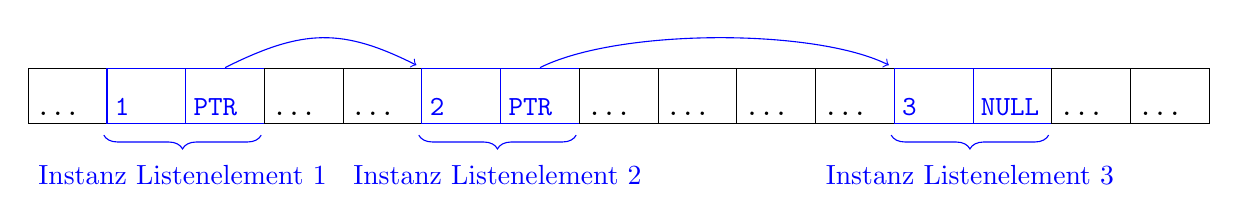
\begin{tikzpicture}
  [ 
    cell/.style={text width=8mm,
    text height=5mm, draw=black, inner sep=1mm},
    ld/.style={draw=blue,shorten >=2pt,->}
  ]
  \node (c01) at ( 0,0) [cell]       {\ttfamily \ldots};
  \node (c02) at ( 1,0) [cell, blue] {\ttfamily 1};
  \node (c03) at ( 2,0) [cell, blue] {\ttfamily PTR};
  \node (c04) at ( 3,0) [cell]       {\ttfamily \ldots};
  \node (c05) at ( 4,0) [cell]       {\ttfamily \ldots};
  \node (c06) at ( 5,0) [cell, blue] {\ttfamily 2};
  \node (c07) at ( 6,0) [cell, blue] {\ttfamily PTR};
  \node (c08) at ( 7,0) [cell]       {\ttfamily \ldots};
  \node (c09) at ( 8,0) [cell]       {\ttfamily \ldots};
  \node (c10) at ( 9,0) [cell]       {\ttfamily \ldots};
  \node (c11) at (10,0) [cell]       {\ttfamily \ldots};
  \node (c12) at (11,0) [cell, blue] {\ttfamily 3};
  \node (c13) at (12,0) [cell, blue] {\ttfamily NULL};
  \node (c14) at (13,0) [cell]       {\ttfamily \ldots};
  \node (c15) at (14,0) [cell]       {\ttfamily \ldots};
  
  \draw [ld] (c03.north) .. controls +(1.0,0.5) and +(-1.0, 0.5) .. (c06.north west);
  \draw [ld] (c07.north) .. controls +(1.0,0.5) and +(-1.0, 0.5) .. (c12.north west);

  \draw [decorate, decoration={brace, amplitude=5pt, mirror}, xshift=-4pt, yshift=0pt, blue]
  		(0.6, -0.5) -- (2.6, -0.5) 
  		node [midway, yshift=-0.5cm]
		(I1) {Instanz Listenelement 1};
  \draw [decorate, decoration={brace, amplitude=5pt, mirror}, xshift=-4pt, yshift=0pt, blue]
  		(4.6, -0.5) -- (6.6, -0.5) 
  		node [midway, yshift=-0.5cm]
		(I2) {Instanz Listenelement 2};
  \draw [decorate, decoration={brace, amplitude=5pt, mirror}, xshift=-4pt, yshift=0pt, blue]
  		(10.6, -0.5) -- (12.6, -0.5) 
  		node [midway, yshift=-0.5cm]
		(I3) {Instanz Listenelement 3};
\end{tikzpicture}
\end{tcolorbox}

Jede Instanz von \texttt{listElement\_t} besteht aus zwei \enquote{Zellen}, die mehr oder minder zufällig im Speicher angeordnet sind. Auch die Reihenfolge ist nicht festgelegt; das dritte Element der Liste kann eine kleinere Adresse haben als das zweite. Dennoch ist die Liste in ihrer Gänze geordnet reproduzierbar, da zu jedem Element bekannt ist, wo der Nachfolger im Speicher zu finden ist. Diese Information ist im Feld \texttt{next} enthalten.

Das letzte Element der Liste -- hier das Dritte -- hat keinen Nachfolger mehr. Daher wird \texttt{next} auf den Wert \texttt{NULL} gesetzt.

Wenn nun ein neues Element in die Liste eingefügt werden soll, so müssen nur drei Schritte ausgeführt werden:
\begin{itemize}
\item Speicher für das neue Element bereit stellen
\item Den Pointer \texttt{next} seines Vorgängers auf das einzufügende Element umleiten
\item Den Pointer \texttt{next} des Einzufügenden Elements auf seinen Nachfolger
\end{itemize}

Wir können dies so verbildlichen:

\begin{tcolorbox}[title=Visualisierung: Einfügen in eine verkettete Liste]
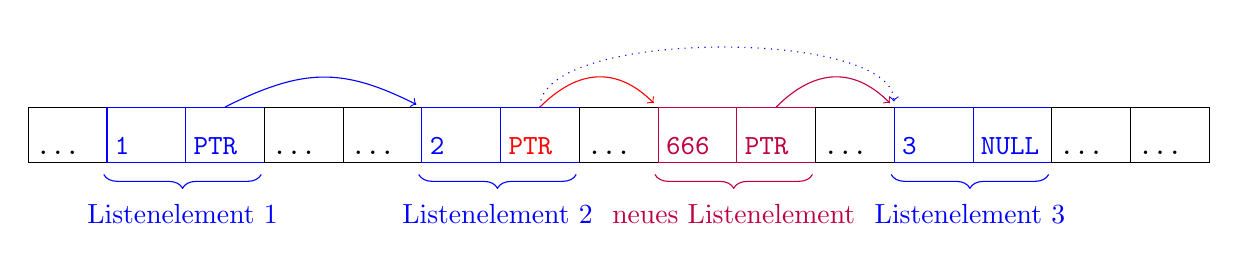
\begin{tikzpicture}
  [ 
    cell/.style={text width=8mm,
    text height=5mm, draw=black, inner sep=1mm},
    ld/.style={draw=blue,shorten >=2pt,->}
  ]
  \node (c01) at ( 0,0) [cell]         {\ttfamily \ldots};
  \node (c02) at ( 1,0) [cell, blue]   {\ttfamily 1};
  \node (c03) at ( 2,0) [cell, blue]   {\ttfamily PTR};
  \node (c04) at ( 3,0) [cell]         {\ttfamily \ldots};
  \node (c05) at ( 4,0) [cell]         {\ttfamily \ldots};
  \node (c06) at ( 5,0) [cell, blue]   {\ttfamily 2};
  \node (c07) at ( 6,0) [cell, blue]   {\ttfamily \textcolor{red}{PTR}};
  \node (c08) at ( 7,0) [cell]         {\ttfamily \ldots};
  \node (c09) at ( 8,0) [cell, purple] {\ttfamily 666};
  \node (c10) at ( 9,0) [cell, purple] {\ttfamily PTR};
  \node (c11) at (10,0) [cell]         {\ttfamily \ldots};
  \node (c12) at (11,0) [cell, blue]   {\ttfamily 3};
  \node (c13) at (12,0) [cell, blue]   {\ttfamily NULL};
  \node (c14) at (13,0) [cell]         {\ttfamily \ldots};
  \node (c15) at (14,0) [cell]         {\ttfamily \ldots};
  
  \draw [ld]         (c03.north) .. controls +(1.0,0.5) and +(-1.0, 0.5) .. (c06.north west);
  \draw [ld, dotted] (c07.north) .. controls +(0.0,1.0) and +(-0.0, 1.0) .. (c12.north west);
  \draw [ld, red]    (c07.north) .. controls +(0.5,0.5) and +(-0.5, 0.5) .. (c09.north west);
  \draw [ld, purple] (c10.north) .. controls +(0.5,0.5) and +(-0.5, 0.5) .. (c12.north west);

  \draw [decorate, decoration={brace, amplitude=5pt, mirror}, xshift=-4pt, yshift=0pt, blue]
  		(0.6, -0.5) -- (2.6, -0.5) 
  		node [midway, yshift=-0.5cm]
		(I1) {Listenelement 1};
  \draw [decorate, decoration={brace, amplitude=5pt, mirror}, xshift=-4pt, yshift=0pt, blue]
  		(4.6, -0.5) -- (6.6, -0.5) 
  		node [midway, yshift=-0.5cm]
		(I2) {Listenelement 2};
  \draw [decorate, decoration={brace, amplitude=5pt, mirror}, xshift=-4pt, yshift=0pt, blue]
  		(10.6, -0.5) -- (12.6, -0.5) 
  		node [midway, yshift=-0.5cm]
		(I3) {Listenelement 3};
  \draw [decorate, decoration={brace, amplitude=5pt, mirror}, xshift=-4pt, yshift=0pt, purple]
  		(7.6, -0.5) -- (9.6, -0.5) 
  		node [midway, yshift=-0.5cm]
		(I4) {neues Listenelement};
\end{tikzpicture}
Ein neues Element (dargestellt in violett) soll in die Liste eingefügt werden. Dazu wird zunächst Speicherplatz reserviert. Die neuen Werte (\texttt{666} sowie der Pointer auf den Nachfolger des einzufügenden Wertes) werden in die entsprechenden Speicherzellen geschrieben. Schließlich wird der Pointer des Vorgängers des eingefügten Listenelements aktualisiert: Er zeigt nun nicht mehr auf den Nachfolger des eingefügten Werts (gepunktete Linie), sondern auf den eingefügten Wert selbst.
\end{tcolorbox}

Solange wir also das erste Element einer Liste kennen, können wir jedes weitere Element erreichen, indem wir \enquote{von Listenelement zu Listenelement springen}\footnote{Natürlich kostet jeder dieser Sprünge Zeit. Wir werden uns hierzu in Abschnitt \ref{sec:linkedListRuntime} mehr Gedanken machen}. Wenn neue Elemente in die Liste eingefügt werden sollen, so muss nur die Speicherstelle ausfindig gemacht werden, die das Listenelement beschreibt, \emph{hinter} das eingefügt werden soll.

Hierbei gibt es noch zwei Spezialfälle: Wenn ein Element an das \emph{Listenende} angefügt werden soll, gibt es keinen Nachfolger des eingefügten Elements. In diesem Fall wird der Pointer \texttt{next} auf \texttt{NULL} gesetzt:

\begin{tcolorbox}[title=Visualisierung: Einfügen an das Ende einer verkettete Liste]
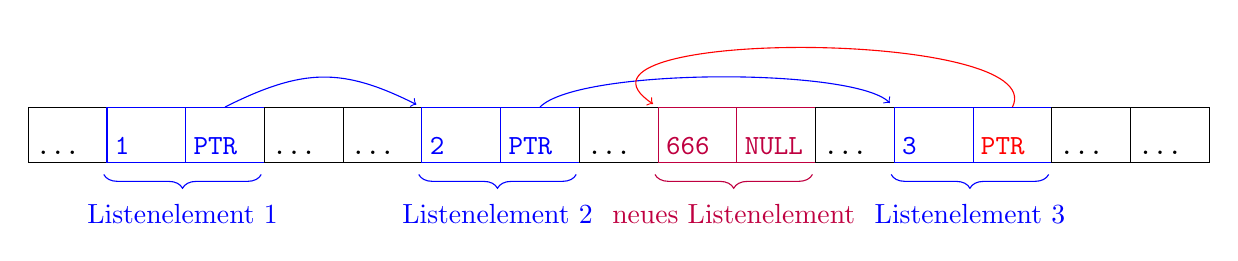
\begin{tikzpicture}
  [ 
    cell/.style={text width=8mm,
    text height=5mm, draw=black, inner sep=1mm},
    ld/.style={draw=blue,shorten >=2pt,->}
  ]
  \node (c01) at ( 0,0) [cell]         {\ttfamily \ldots};
  \node (c02) at ( 1,0) [cell, blue]   {\ttfamily 1};
  \node (c03) at ( 2,0) [cell, blue]   {\ttfamily PTR};
  \node (c04) at ( 3,0) [cell]         {\ttfamily \ldots};
  \node (c05) at ( 4,0) [cell]         {\ttfamily \ldots};
  \node (c06) at ( 5,0) [cell, blue]   {\ttfamily 2};
  \node (c07) at ( 6,0) [cell, blue]   {\ttfamily PTR};
  \node (c08) at ( 7,0) [cell]         {\ttfamily \ldots};
  \node (c09) at ( 8,0) [cell, purple] {\ttfamily 666};
  \node (c10) at ( 9,0) [cell, purple] {\ttfamily NULL};
  \node (c11) at (10,0) [cell]         {\ttfamily \ldots};
  \node (c12) at (11,0) [cell, blue]   {\ttfamily 3};
  \node (c13) at (12,0) [cell, blue]   {\ttfamily \textcolor{red}{PTR}};
  \node (c14) at (13,0) [cell]         {\ttfamily \ldots};
  \node (c15) at (14,0) [cell]         {\ttfamily \ldots};
  
  \draw [ld]         (c03.north) .. controls +(1.0,0.5) and +(-1.0, 0.5) .. (c06.north west);
  \draw [ld]         (c07.north) .. controls +(0.5,0.5) and +(-0.5, 0.5) .. (c12.north west);
  \draw [ld, red]    (c13.north) .. controls +(0.5,1.0) and +(-1.5, 1.0) .. (c09.north west);

  \draw [decorate, decoration={brace, amplitude=5pt, mirror}, xshift=-4pt, yshift=0pt, blue]
  		(0.6, -0.5) -- (2.6, -0.5) 
  		node [midway, yshift=-0.5cm]
		(I1) {Listenelement 1};
  \draw [decorate, decoration={brace, amplitude=5pt, mirror}, xshift=-4pt, yshift=0pt, blue]
  		(4.6, -0.5) -- (6.6, -0.5) 
  		node [midway, yshift=-0.5cm]
		(I2) {Listenelement 2};
  \draw [decorate, decoration={brace, amplitude=5pt, mirror}, xshift=-4pt, yshift=0pt, blue]
  		(10.6, -0.5) -- (12.6, -0.5) 
  		node [midway, yshift=-0.5cm]
		(I3) {Listenelement 3};
  \draw [decorate, decoration={brace, amplitude=5pt, mirror}, xshift=-4pt, yshift=0pt, purple]
  		(7.6, -0.5) -- (9.6, -0.5) 
  		node [midway, yshift=-0.5cm]
		(I4) {neues Listenelement};
\end{tikzpicture}
Beim Einfügen an das Listenende muss wieder der Pointer \texttt{next} des Vorgängers aktualisiert werden. Das neu eingefügte Wert erhält als Nachfolger \texttt{NULL}.\\
Beachten Sie, dass die Anordnung im Speicher nicht zwingend die Reihenfolge der Liste wiedergibt: auch, wenn das neue Listenelement im Speicher zwischen Element 2 und 3 angeordnet ist, handelt es sich um das Listenende (Ordnung durch die Pointer, hier visualisiert als Pfeile).
\end{tcolorbox}

Der andere Spezialfall tritt ein, wenn an den \emph{Anfang} der Liste ein Wert eingefügt werden soll. In diesem Fall müssen wir in der Speicherstruktur unserer Liste keine Pointer aktualisieren. Es ändert sich aber der \enquote{Einstiegspunkt}: Da wir nur \enquote{vorwärts} in unserer Liste weiter springen können, müssen wir als \emph{handle} die Adresse des eingefügten Elements speichern.

\begin{tcolorbox}[title=Visualisierung: Einfügen an den Anfang einer verkettete Liste]
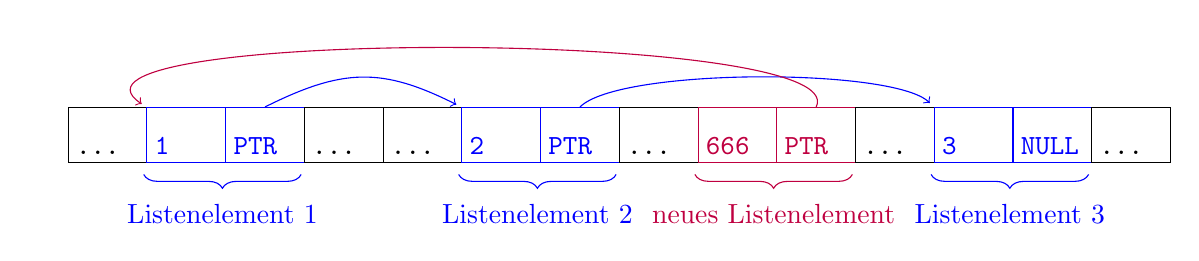
\begin{tikzpicture}
  [ 
    cell/.style={text width=8mm,
    text height=5mm, draw=black, inner sep=1mm},
    ld/.style={draw=blue,shorten >=2pt,->}
  ]
  \node (c01) at ( 0,0) [cell]         {\ttfamily \ldots};
  \node (c02) at ( 1,0) [cell, blue]   {\ttfamily 1};
  \node (c03) at ( 2,0) [cell, blue]   {\ttfamily PTR};
  \node (c04) at ( 3,0) [cell]         {\ttfamily \ldots};
  \node (c05) at ( 4,0) [cell]         {\ttfamily \ldots};
  \node (c06) at ( 5,0) [cell, blue]   {\ttfamily 2};
  \node (c07) at ( 6,0) [cell, blue]   {\ttfamily PTR};
  \node (c08) at ( 7,0) [cell]         {\ttfamily \ldots};
  \node (c09) at ( 8,0) [cell, purple] {\ttfamily 666};
  \node (c10) at ( 9,0) [cell, purple] {\ttfamily PTR};
  \node (c11) at (10,0) [cell]         {\ttfamily \ldots};
  \node (c12) at (11,0) [cell, blue]   {\ttfamily 3};
  \node (c13) at (12,0) [cell, blue]   {\ttfamily NULL};
  \node (c14) at (13,0) [cell]         {\ttfamily \ldots};
  
  \draw [ld]         (c03.north) .. controls +(1.0,0.5) and +(-1.0, 0.5) .. (c06.north west);
  \draw [ld]         (c07.north) .. controls +(0.5,0.5) and +(-0.5, 0.5) .. (c12.north west);
  \draw [ld, purple] (c10.north) .. controls +(0.5,1.0) and +(-1.5, 1.0) .. (c02.north west);

  \draw [decorate, decoration={brace, amplitude=5pt, mirror}, xshift=-4pt, yshift=0pt, blue]
  		(0.6, -0.5) -- (2.6, -0.5) 
  		node [midway, yshift=-0.5cm]
		(I1) {Listenelement 1};
  \draw [decorate, decoration={brace, amplitude=5pt, mirror}, xshift=-4pt, yshift=0pt, blue]
  		(4.6, -0.5) -- (6.6, -0.5) 
  		node [midway, yshift=-0.5cm]
		(I2) {Listenelement 2};
  \draw [decorate, decoration={brace, amplitude=5pt, mirror}, xshift=-4pt, yshift=0pt, blue]
  		(10.6, -0.5) -- (12.6, -0.5) 
  		node [midway, yshift=-0.5cm]
		(I3) {Listenelement 3};
  \draw [decorate, decoration={brace, amplitude=5pt, mirror}, xshift=-4pt, yshift=0pt, purple]
  		(7.6, -0.5) -- (9.6, -0.5) 
  		node [midway, yshift=-0.5cm]
		(I4) {neues Listenelement};
\end{tikzpicture}
Beim Einfügen an den Listenanfang muss keines der bestehenden Listenelemente aktualisiert werden. Da jedoch nur Elemente in \enquote{Vorwärtsrichtung} (der Pfeile) erreicht werden können, ist unser Einstiegspunkt für die Listenverwaltung das neu eingefügte Element.
\end{tcolorbox}

Auch das Löschen von Werten aus der Liste ist jetzt leicht umsetzbar: Wir suchen den \emph{Vorgänger} des zu löschenden Elements, ändern seinen Pointer auf den \emph{Nachfolger} des zu löschenden Elements, und vergessen nicht, den Speicher freizugeben:

\begin{tcolorbox}[title=Visualisierung: Löschen aus einer verketteten Liste]
\begin{tikzpicture}
  [ 
    cell/.style={text width=8mm,
    text height=5mm, draw=black, inner sep=1mm},
    ld/.style={draw=blue,shorten >=2pt,->}
  ]
  \node (c01) at ( 0,0) [cell]         {\ttfamily \ldots};
  \node (c02) at ( 1,0) [cell, blue]   {\ttfamily 1};
  \node (c03) at ( 2,0) [cell, blue]   {\ttfamily PTR};
  \node (c04) at ( 3,0) [cell]         {\ttfamily \ldots};
  \node (c05) at ( 4,0) [cell]         {\ttfamily \ldots};
  \node (c06) at ( 5,0) [cell, blue]   {\ttfamily 2};
  \node (c07) at ( 6,0) [cell, blue]   {\ttfamily \textcolor{red}{PTR}};
  \node (c08) at ( 7,0) [cell]         {\ttfamily \ldots};
  \node (c09) at ( 8,0) [cell, grey]   {\ttfamily 666};
  \node (c10) at ( 9,0) [cell, grey]   {\ttfamily PTR};
  \node (c11) at (10,0) [cell]         {\ttfamily \ldots};
  \node (c12) at (11,0) [cell, blue]   {\ttfamily 3};
  \node (c13) at (12,0) [cell, blue]   {\ttfamily NULL};
  \node (c14) at (13,0) [cell]         {\ttfamily \ldots};
  \node (c15) at (14,0) [cell]         {\ttfamily \ldots};
  
  \draw [ld]         (c03.north) .. controls +(1.0,0.5) and +(-1.0, 0.5) .. (c06.north west);
  \draw [ld, red]    (c07.north) .. controls +(0.0,1.0) and +(-0.0, 1.0) .. (c12.north west);
  \draw [ld, dotted] (c07.north) .. controls +(0.5,0.5) and +(-0.5, 0.5) .. (c09.north west);
  \draw [ld, dotted] (c10.north) .. controls +(0.5,0.5) and +(-0.5, 0.5) .. (c12.north west);

  \draw [decorate, decoration={brace, amplitude=5pt, mirror}, xshift=-4pt, yshift=0pt, blue]
  		(0.6, -0.5) -- (2.6, -0.5) 
  		node [midway, yshift=-0.5cm]
		(I1) {Listenelement 1};
  \draw [decorate, decoration={brace, amplitude=5pt, mirror}, xshift=-4pt, yshift=0pt, blue]
  		(4.6, -0.5) -- (6.6, -0.5) 
  		node [midway, yshift=-0.5cm]
		(I2) {Listenelement 2};
  \draw [decorate, decoration={brace, amplitude=5pt, mirror}, xshift=-4pt, yshift=0pt, blue]
  		(10.6, -0.5) -- (12.6, -0.5) 
  		node [midway, yshift=-0.5cm]
		(I3) {Listenelement 3};
  \draw [decorate, decoration={brace, amplitude=5pt, mirror}, xshift=-4pt, yshift=0pt, grey]
  		(7.6, -0.5) -- (9.6, -0.5) 
  		node [midway, yshift=-0.5cm]
		(I4) {gelöschtes Element};
\end{tikzpicture}
Beim Löschen eines Elements -- hier des Eintrags zwischen Element 2 und Element 3 -- muss lediglich der Pointer \texttt{next} des \emph{Vorgängers} aktualisiert und der Speicher freigegeben werden.
\end{tcolorbox}

Auch hier ergeben sich Spezialfälle für Löschen am Listenanfang bzw. am Listenende. Sie können sich jetzt leicht vorstellen, wie diese Fälle aussehen. Im folgenden Abschnitt werden wir diese mit Codebeispielen genauer betrachten.

\section{Aufbau einer Bibliothek zur Verwaltung von Linked Lists}
Die im letzten Abschnitt besprochenen Ideen haben bereits einige Komplexität. Wir wollen nicht für jedes Projekt, in dem wir diese Technik brauchen, komplett von Null weg beginnen. Daher schreiben wir uns eine \emph{Bibliothek}, in der wir die Routinen zur Verwaltung einer Linked List in allgemeiner Form ablegen. 

\subsection{Die Datentypen}
Da sich der Einstiegspunkt in unsere Liste ändern kann, führen wir einen weiteren Datentyp (eine weitere \mintinline{c}{struct}) ein, in dem wir diesen Einstiegspunkt und andere Daten speichern. Diesen neuen Datentyp wollen wir \texttt{linkedlist\_t} nennen.

Während sich durch unsere Operationen (\eg Einfügen in und Löschen aus der Liste) der Einstiegspunkt ändern kann, bleibt die Speicherstelle der Variable vom Typ \texttt{linkedlist\_t} konstant. Wenn wir unsere Routinen so gestalten, dass diese diese \enquote{Verwaltungs-Variable} aktuell halten, können wir für die Verwendung unserer Liste ihre innere Struktur \enquote{vergessen}. Wir erledigen einmal die Aufgaben Speicherverwaltung und Listen-Management. Für unser eigentliches Projekt dann können wir einfach die Routinen unserer Bibliothek verwenden und müssen keine Gedanken mehr darauf aufwenden, ob alle Pointer auf die richtigen Speicherstellen zeigen.

Wir wollen mit unserer Bibliothek Listen beliebigen Datentyps anlegen. Dies umfasst sowohl die \emph{primitiven Datentypen} (\mintinline{c}{int}, \mintinline{c}{double}, ...) als auch selbst erstellte \mintinline{c}{struct}s. Daher werden wir den Datentyp von \texttt{data} in der \texttt{listElement\_t} auf \mintinline{c}{void *} abändern. Das heißt, wir speichern \enquote{in der linken Zelle} unserer Listenelemente nicht mehr den Wert selbst, sondern nur, wo im Speicher sich der tatsächliche Wert befindet. Um die Ausgabe der Liste auf dem Bildschirm zu vereinfachen, fügen wir \texttt{linkedlist\_t} einen Funktionszeiger hinzu. Dieser soll eine Funktion benennen, die den Datentyp der Liste gut auf dem Bildschirm ausgeben kann.

Aus praktischen Gründen speichern wir außerdem noch mit, wie viele Elemente unsere Liste im Moment hat. Diese Information ist zwar durch Nachverfolgen der Pointer zugänglich; bei langen Listen dauert es aber, bis man durch die gesamte Kette gesprungen ist. Schließlich führen wir noch den Wahrheitswert \texttt{memoryAutoManaged} ein, dessen Funktion ich weiter unten genauer erläutere.

Aus diesen Überlegungen ergeben sich diese Datentypen:
\begin{codebox}[Datentypen für Listenelemente und Verwaltungsvariable einer Linked List]
\begin{minted}[linenos]{c}
typedef struct listElement_struct {
  void *                      data;
  struct listElement_struct * next;
} listElement_t;

typedef struct {
  listElement_t * first;
  int             size;
  
  int             memoryAutoManaged;
  void (*printElement)(void *);
} linkedList_t;
\end{minted}
\end{codebox}

Da dies bislang nur \emph{Definitionen} waren, gehört dieser Code in eine Header-Datei. Wir wollen sie \texttt{linkedlist.h} nennen. Der folgende Code soll in einer Moduldatei mit dem Namen \texttt{linkedlist.c} gespeichert sein.

\subsection{Aufbau und Bereinigung der Liste -- Constructor und Destructor}
Um mit der Liste Arbeiten zu können, muss zuerst ein definierter Ausgangszustand geschaffen werden. Hier werden wir bereits Speicherplatz allozieren müssen, daher sollten wir uns im selben Abschnitt der Entwicklung auch bereits Gedanken um die Freigabe des allozierten Speichers machen.

Routinen, die Speicherstrukturen vorbereiten werden \emph{Constructors} genannt. Prozeduren, die Speicher wieder freigeben, bezeichnen wir als \emph{Destructors}. Wir entwickeln hier also den Constructor \texttt{make\_linkedList} und den Destructor \texttt{free\_linkedList}.

Da jede Einfügung oder Löschung den Einstiegspunkt (\texttt{first}) und die Zahl der Elemente (\texttt{size}) ändern können, müssen unsere Routinen mit Pointern auf die Verwaltungs-Variable arbeiten. Damit wir vermeiden können, in jedem Aufruf der Routinen unserer Bibliothek einen Adress-Operator \texttt{\&} setzen zu müssen, konzipieren wir gleich den Constructor so, dass ein Pointer erzeugt wird:

\begin{codebox}[Constructor einer Linked List]
\begin{minted}[linenos]{c}
#include <stdio.h>
#include <stdlib.h>
#include <string.h>
#include "linkedlist.h"

linkedList_t * make_linkedList () {
  linkedList_t * reVal = malloc(sizeof(*reVal));
  if (!reVal) {
    printf("Fehler: Speicher konnte nicht alloziert werden\n");
    return NULL;
  }
  
  reVal->first             = NULL;
  reVal->size              = 0;
  reVal->printElement      = NULL;
  reVAl->memoryAutoManaged = 0;
  
  return reVal;
}
\end{minted}
\end{codebox}

Alle Elemente der Verwaltungsstruktur werden zunächst auf null gesetzt. Damit sind zufällige Effekte von \enquote{Resten im Speicher} ausgeschlossen.

Der Destructor muss alle Elemente der Liste löschen und schließlich den Speicherplatz für die Verwaltungsstruktur vom Typ \texttt{linkedList\_t} selbst freigeben. Da wir später ohnehin einzelne Listen-Elemente löschen wollen werden, können wir für diese Aufgabe auf die (noch nicht existierende) Funktion \texttt{delete\_from\_linkedList} zurückgreifen. Dieser Funktion übergeben wir den Index des zu löschenden Listenelements. Wenn wir oft genug das erste Element der Liste entfernen, geben wir am Ende allen Speicher frei. Der Code lässt sich folgendermaßen schreiben:

\begin{codebox}[Destructor einer Linked List]
\begin{minted}[linenos, firstnumber=last]{c}
void free_linkedList(linkedList_t * list) {
  while (list->size) {
    delete_from_linkedList(list, 0);
  }
  
  free(list);
}
\end{minted}
\end{codebox}

\subsection{Sprünge durch die Liste}
Es wäre naheliegend nun die Funktion \texttt{delete\_from\_linkedList} zu schreiben. Da wir für jede Veränderung der Liste jedoch zuerst ein bestimmtes Listenelement \enquote{finden} müssen, bietet es sich an, zuerst diese Sprünge durch die Liste umzusetzen. Wir entwickeln also eine Routine, der wir einen Index mitteilen, und die das zugehörige Listenelement ausfindig macht:

\begin{codebox}[Sprung zu einem bestimmten Element einer Linked List]
\begin{minted}[linenos, firstnumber=last]{c}
listElement_t * get_linkedList_element(linkedList_t * list, int index) {
  if (index < 0 || index >= list->size) {
    printf("Fehler: ungültiger Index\n");
    return NULL;
  }
  
  listElement_t * element = list->first;
  for (int i=0; i<index; i++) {
    element = element->next;
  }
  
  return element;
}
\end{minted}
\end{codebox}

\subsection{Löschen und Einfügen in die Liste}
Mit diesem Werkzeug können wir nun endlich das Löschen von Elementen aus der Liste angehen; im selben Schritt werden wir uns dann auch mit dem Einfügen in die Liste beschäftigen.

\begin{codebox}[Löschen aus einer Linked List]
\begin{minted}[linenos, firstnumber=last]{c}
int delete_from_linkedList(linkedList_t * list, int index) {
  if (index < 0 || index >= list->size) {
    printf("Fehler: ungültiger Index\n");
    return -1;
  }
  
  listElement_t * prev, * self, * next;
  
  if (index == 0) {
    prev = NULL;
    self = list->first;
    list->first = self->next;
    
  } else {
    prev = get_linkedList_element(list, index - 1);
    self = prev->next;
  }
  
  next = self->next;
  if (prev) {prev->next = next;}
  
  if (list->memoryAutoManaged) {free(self->data);}
  free(self);
  
  return --list->size;
}
\end{minted}
\end{codebox}

Wir beschaffen uns zunächst die Adressen des zu löschenden Elements, sowie die seines Vor- als auch Nachgängers (Variablen \texttt{self}, \texttt{prev} und \texttt{next}.) Wenn das erste Element der Liste gelöscht werden soll (wenn \texttt{index} gleich \texttt{0} ist), existiert kein Vorgänger. Wir behandeln diesen Fall gesondert (\mintinline{c}{if} in Zeile 48). Hier beachten wir auch, dass sich der Einstiegspunkt in unsere Liste ändern wird (Zeile 51). Ansonsten benutzen wir die soeben geschriebene Funktion \texttt{get\_linkedList\_element}, um das zu löschende Element ausfindig zu machen. In jedem Fall ist sein Nachfolger über \texttt{self->next} ausfindig zu machen. Da wir mit dem \mintinline{c}{if} in Zeile 41 prüfen, ob ein \enquote{sinnvoller} \texttt{index} übergeben wurde, ist auch sichergestellt, dass \texttt{self} von \texttt{NULL} verschieden ist. (Sie erinnern sich, dass \texttt{self->next} eine Kurzform für \texttt{(*self).next} ist, und dass \texttt{*pointer} verboten ist, wenn \texttt{pointer == NULL}.)

Wird \texttt{self} gelöscht, so soll das Listenelement an der Stelle \texttt{prev} entweder auf den Nachfolger von \texttt{self} verweisen, wenn ein solcher existiert, oder den Wert \texttt{NULL} erhalten, wenn es nach der Löschung das letzte Element der Liste ist.

Wir können davon ausgehen, dass unsere Liste zuvor in einem intakten Zustand war. Die Variable \texttt{next} erhält damit in Zeile 58 als Wert entweder einen Pointer auf ein Element unserer Liste, oder den Wert \texttt{NULL}, falls \texttt{self} auf das Ende der Liste zeigt. Wir müssen also keine Fallunterscheidung für Mitte und Ende der Liste machen.

Allerdings kann es sein, dass das erste Element der Liste gelöscht wird, und daher \texttt{prev == NULL}. Nur wenn dies nicht der Fall ist, kann ein Pointer aktualisiert werden -- wir schrebein in Zeile 59 ein \mintinline{c}{if}.

Im vorigen Kapitel bei der \texttt{stringlist} sind wir auf das Problem gestoßen, dass der Speicherplatz für die Nutzdaten (dort also für die einzelnen Strings) von den Routinen der Stringlist komplett verwaltet werden sollte. Wir wollen hier einen ähnlichen Weg gehen, jedoch ein zusätzliches Szenario bedenken:

Es ist möglich, dass wir in unserem Projekt mehr als eine LinkedList benutzen. Die beiden Listen könnten sich Elemente teilen, \ie dasselbe Element kommt in zwei Listen vor. (Denken Sie beispielsweise an die Verwaltung einer Firma. Eine Liste könnte alle Angestellten sein, eine speichert alle Angestellten, die in der Abteilung IT arbeiten). Wenn nun die erste Liste freigegeben wird (\eg die Liste \emph{aller} Angestellten), so wird auch der Speicher aller Nutzdaten freigegeben -- selbst der Speicher, der in der zweiten Liste (die der Angestellten in der IT) registrierten Nutzdaten. 

Um dieses Problem zu umgehen, haben wir den \enquote{Schalter} \texttt{memoryAutoManaged} in \texttt{linkedList\_t} eingebaut. Nutzdaten werden nur freigegeben, wenn die aktuelle Liste die Nutzdaten auch \enquote{besitzen} soll. In Zeile 61 wird daher nur für diesen Fall der Speicher der Nutzdaten freigegeben.

Da nun alle Pointer aktualisiert sind, können wir endlich auch den Speicher des Listenelements freigeben (Zeile 62) und weiter unserer Verwaltungs-Variablen mitteilen, dass sich die Länge unserer Liste geändert hat (Zeile 64). 

Eine Liste hat immer eine nicht-negative Länge. Wir nutzen diese Information, und geben als Rückgabewert entweder die neue Länge der Liste zurück, wenn die Löschung erfolgreich war, oder einen negativen Wert, um anzudeuten, dass ein Fehler aufgetreten ist.

Betrachten wir nun Einfügungen in die Liste:

\begin{codebox}[Einfügen in eine Linked List]
\begin{minted}[linenos, firstnumber=last]{c}
int add_to_linkedList(
  linkedList_t * list, int index, 
  void * newData, size_t bytes
) {
  if (index < 0 || index > list->size) {
    printf("Fehler: ungültiger Index\n");
    return -1;
  }
\end{minted}
\end{codebox}
%
\begin{codebox}[]
\begin{minted}[linenos, firstnumber=last]{c}
  listElement_t * prev, * self, * next;
  
  self = malloc(sizeof(*self));
  if (!self) {
    printf("Fehler: Speicher konnte nicht alloziert werden\n");
    return -1;
  }
  
  if (list->memoryAutoManaged) {
    self->data = malloc(bytes);
    if (!self->data) {
      printf("Fehler: Speicher konnte nicht alloziert werden\n");
      free(self);
      return -1;
    }
    memcpy(self->data, newData, bytes);
    
  } else {
    self->data = newData;
  }
  
  if (index == 0) {
    prev = NULL;
    next = list->first;
    list->first = self;
    
  } else {
    prev = get_linkedList_element(list, index - 1);
    next = prev->next;
  }
  
  if (prev) {prev->next = self;}
  self->next = next;
  
  return ++list->size;
}
\end{minted}
\end{codebox}

Der Test, ob der übergebene \texttt{index} sinnvoll ist, sieht fast genauso aus wie schon in der Routine zum Löschen; jedoch erlauben wir hier Werte bis \emph{einschließlich} der Länge der Liste, da es auch möglich sein soll, Werte an ihr Ende anzuhängen.

Wir reservieren also Speicher für unser Listenelement (Zeile 76). Für die tatsächlichen Nutzdaten betrachten wir wieder den Status des \enquote{Schalters} \texttt{memoryAutoManaged}.

Wenn unsere Liste die ihr zugeordneten Elemente \emph{komplett selbst verwalten soll}, legen wir eine Kopie der übergebenen Nutzdaten (\texttt{newData}) an, und verhindern so, dass Daten doppelt freigegeben werden (Zeilen 82 bis 89). Da dies bei großen Nutzdaten jedoch viel Zeit beanspruchen kann, erlauben wir auch, dass lediglich die Speicheradresse der Nutzdaten in unsere Liste übernommen wird, ohne eine Kopie anzulegen (Zeile 92).

In Zeile 95 treffen wir wieder auf den Sonderfall, dass an den Listenanfang eingefügt werden soll. Wir notieren, dass es keinen Vorgänger gibt, der aktualisiert werden muss, und merken uns den Nachfolger: das vormals erste Element der Liste. Außerdem aktualisieren wir den Einstiegspunkt.

Für den allgemeinen Fall dagegen machen wir einfach das Listenelement vor dem Einfügepunkt ausfindig (Zeile 101). Sein Nachfolger ist wieder entweder ein Pointer auf ein Listenelement oder der Wert \texttt{NULL} falls \texttt{index} auf das Listenenede verweist -- also für alle denkbaren Szenarios der richtige Wert. Den so gefundenen Nachfolger \texttt{next} weisen wir dann als Nachfolger von \texttt{self} zu (Zeile 106), und aktualisieren auch den Vorgänger, falls ein solcher existiert (Zeile 105).

\subsection{Ausgeben der gesamten Liste}
Als Beispiel für die Aufgaben, die mit einer Liste erledigt werden müssen wollen wir alle Elemente auf dem Bildschirm ausgeben. Wir wissen zwar nicht, welche Struktur ein einzelnes Listenelement hat (unsere Nutzdaten sind ein \mintinline{c}{void *}), aber wir kennen eine Funktion, die mit diesen Daten umzugehen weiß -- die \texttt{printElement} aus \texttt{linkedList\_t}! Damit gestaltet sich diese Aufgabe als sehr leicht:

\begin{codebox}[Alle Listenelemente ausgeben]
\begin{minted}[linenos, firstnumber=last]{c}
void print_all_from_linkedlist(linkedList_t * list) {
  listElement_t * element = list->first;
  while (element != NULL) {
    list->printElement(element->data);
    element = element->next;
  }
}
\end{minted}
\end{codebox}

\subsection{Der Komplette Header}
In den vorigen Abschnitten haben wir den Code unserer Bibliothek kennen gelernt. Damit die Routinen in unserem eigentlichen Projekt zur Verfügung stehen, müssen wir den Header um die Deklaration der Routinen ergänzen. Vollständig lautet der Header also:

\begin{codebox}[Kompletter Header \texttt{linkedlist.h}]
\begin{minted}[linenos]{c}
#include <stdlib.h>

typedef struct listElement_struct {
  void *                      data;
  struct listElement_struct * next;
} listElement_t;

typedef struct {
  listElement_t * first;
  int             size;
  
  int             memoryAutoManaged;
  void (*printElement)(void *);
} linkedList_t;
\end{minted}
\end{codebox}
%
\begin{codebox}[]
\begin{minted}[linenos, firstnumber=last]{c}
linkedList_t * make_linkedList ();
void           free_linkedList(linkedList_t * list);

listElement_t * get_linkedList_element(linkedList_t * list, int index);

int delete_from_linkedList(linkedList_t * list, int index);
int add_to_linkedList(
  linkedList_t * list, int index, 
  void * newData, size_t bytes
);

void print_all_from_linkedlist(linkedList_t * list);
\end{minted}
\end{codebox}

Aller weiterer Code, wie Sie ihn gerade gesehen haben, ist im Modul \texttt{linkedlist.c} zu finden.

\subsection{Anwendungsbeispiel}
Wir haben nun die wichtigsten Routinen für die Arbeit mit einer Linked List fertig gestellt. Natürlich kann man den Funktionsumfang noch beliebig erweitern (Durchsuchen, Sortieren, Werte tauschen, ...). Hier wollen wir uns aber darauf beschränken, die gezeigten Routinen in Anwendung zu sehen.

Wir legen eine Liste aus zwei Arbeitnehmern einer Firma an. Wir halten den Schalter \texttt{memoryAutoManaged} zunächst auf \emph{false}, um unnötiges Kopieren zu verhindern. Nach dem Befüllen stellen wir den Schalter auf \emph{true}, um eine automatische Freigabe des Speichers für die gesamte Liste zu erreichen.

\begin{codebox}[Anwendungsbeispiel: Angestellte in einer Linked List]
\begin{minted}[linenos]{c}
#include <stdio.h>
#include <string.h>

#include "linkedlist.h"

// ========================================================================= //

typedef struct {
  char   firstName [20];
  char   lastName  [20];
  char   department[20];
  double salary;
} employee_t;

void printEmployee(void * employee) {
  printf("%20s | %20s | %20s | %8.2lf\n",
    (employee_t *) employee->firstName,
    (employee_t *) employee->lastName,
    (employee_t *) employee->department,
    (employee_t *) employee->salary
  );
}

// ========================================================================= //
\end{minted}
\end{codebox}
%
\begin{codebox}[]
\begin{minted}[linenos, firstnumber=last]{c}
int main () {
  linkedList_t * list = make_linkedList();
  
  list->memoryAutoManaged = 0;
  list->printElement = printEmployee;
  
  employee_t * emp = malloc(sizeof(*emp));
    strcpy(emp->firstName , "Vanessa");
    strcpy(emp->lastName  , "Schmetterling");
    strcpy(emp->department, "Betriebsarzt");
    emp->salary     = 7000.0;
  add_to_linkedList(list, 0, emp, 0);
  
  emp = malloc(sizeof(*emp));
    strcpy(emp->firstName , "Rebecka");
    strcpy(emp->lastName  , "Rein");
    strcpy(emp->department, "R&D");
    emp->salary     = 420.69;
  add_to_linkedList(list, 0, emp, 0);
  
  printf(
    "%20s | %20s | %20s | %8s\n",
    "Vorname",
    "Nachname",
    "Abteilung",
    "Lohn"
  );
  printf(
    "---------------------+-"
    "---------------------+-"
    "---------------------+-"
    "--------\n"
  );
  
  print_all_from_linkedlist(list);
  
  list->memoryAutoManaged = 1;
  free_linkedList(list);
}
\end{minted}
\end{codebox}

\begin{cmdbox}[Ausgabebeispiel: Angestellte in einer Linked List]
\begin{minted}{text}
             Vorname |             Nachname |            Abteilung |     Lohn
---------------------+----------------------+----------------------+---------
             Rebecka |                 Rein |                  R&D |   420.69
             Vanessa |        Schmetterling |         Betriebsarzt |  7000.00
\end{minted}
\end{cmdbox}


\section{Einsatzbereiche der Linked List: Vor- und Nachteile} \label{sec:linkedListRuntime}
Der Verwaltungsaufwand von Linkedlists ist größer als der von einfachen Arrays. Zugriffe auf einzelne Elemente erfordern bereits Funktionsaufrufe, und die ganze Struktur macht komplexe Überlegungen zum Speicher-Management nötig. Wann also ist dieser Aufwand gerechtfertigt?

Wir hatten gesehen, dass das Einfügen von Werten in die Mitte der Liste und insbesondere an den Listenanfang besonders einfach geht, da kein Kopieren oder Verschieben von Werten notwendig wird. Solche Aufgaben, bei denen also häufig Elemente in Listen eingeschoben und daraus entfernt werden, können sehr effizient mit Linked Lists erledigt werden.

Das \emph{Iterieren} über \emph{alle} Elemente der Liste ist mit vertretbarem Aufwand zu meistern und hat kein bedeutend schlechteres Laufzeitverhalten als das Bearbeiten aller Elemente eines einfachen Arrays. Im einen Fall springt man jeweils von einem Listenelement zu seinem Nachfolger; im anderen Fall erhöht man einen Index.

Wo \emph{wahlfreier Zugriff} gefordert ist, \ie wo die Reihenfolge der Indizes, auf die man zugreift, nicht der Reihenfolge der Liste entspricht, ist das Verhalten der Linked List klar schlechter als das von Arrays.

Es hängt also vom Anwendungsfall ab: Welche Arten von Aufgaben sollen mit der Liste erledigt werden? Wie wird auf die Listenelemente zugegriffen? Abhängig von der Antwort auf diese Fragen kann die Wahl auf klassische Arrays, Linked Lists oder ganz andere Speicherstrukturen fallen.

Der Vorzeige-Anwendungsfall für Linked Lists sind sogenannte \emph{FIFOs} (englisch: \emph{first in, first out}). Stellen Sie sich einen Stapel vor. Sie können oben auf den Stapel Elemente (Aufgaben) legen; diese werden dann in der umgekehrten Reihenfolge bearbeitet, in der sie auf den Stapel gelegt wurden, \ie das zuletzt eingefügte Element wird als erstes vom Stapel genommen.

In der Vorlesung \emph{Algorithmen \& Datenstrukturen} der Universität Regensburg werden Sie hierzu mehr Details erfahren und auch Strukturen kennen lernen, die auf den Ideen der Linked List aufbauen. Diese Strukturen können zusätzliche Funktionalität bieten (\eg durchsuchbare Bäume) oder für bestimmte Anwendungsfälle optimiert sein (\eg \emph{priority queues}, die besonders schnellen Zugriff auf das größte Element einer Liste erlauben.)

Linked Lists und andere Speicherstrukturen gehören zum Standard-Repertoire des Programmierens. Während Sie die zugrunde liegenden Konzepte verstehen und umsetzen können sollten, werden Sie in der praktischen Anwendung \idR keine Linked Lists selbst schreiben, sondern vorgefertigte Lösungen anderer KollegInnen auf Ihre Projekte anwenden. Beispielsweise können Sie in C die SGLIB verwenden. Siehe hierzu \url{http://sglib.sourceforge.net/}.

\begin{plusbox}[Die Containers-Library in C++]
Der letzte Absatz gilt umso mehr für C++: Die Aufgabe, Daten effizient im Speicher zu behalten und Schnittstellen für Zugriffe bestimmter Art zu implementieren wurde in der STL (Standard Library) für eine Reihe von Szenarios sehr effizient umgesetzt und kann von jedem/jeder ProgrammiererIn genutzt werden.\\
Linked Lists stehen dort in der Klasse \texttt{std::queue} bwz. als \texttt{std::forward\_list} zur Verfügung. Verwandt damit ist der \texttt{std::stack} (LIFO, also \emph{last in, first out}) und die \texttt{std::deque} (double-ended queue).\\
Siehe dazu \url{https://en.cppreference.com/w/cpp/container}
\end{plusbox}